\documentclass[10pt]{beamer}
\usetheme[height=10mm]{Rochester}
% \beamertemplatenavigationsymbolsempty

\usepackage[czech]{babel}

\AtBeginDocument{\renewcommand\vec{\mathbf}}
\usepackage[version=4]{mhchem}
\usepackage{siunitx}
\sisetup{
	locale               = DE,
	inter-unit-product   = \ensuremath{{}\cdot{}},
	list-units           = single,
	list-separator       = {; },
	list-final-separator = \text{ a },
	list-pair-separator  = \text{ a },
	range-phrase         = \text{ až },
	range-units          = single,
	detect-all,                            % Use sans-serif
}
\DeclareSIUnit\arbunit{rel.~j.}
\DeclareSIUnit\atmosphere{atm}

\usepackage{graphicx}
\graphicspath{
	{img/}
}
\usepackage[outdir=build/plots/]{epstopdf}
\usepackage{tikz}

\usetikzlibrary{arrows.meta}
\usetikzlibrary{bending}
\usetikzlibrary{positioning}

\tikzset{
	level/.style = {},
	transition/.style = {
		thick,
		arrows = {-Latex},
	}
}

\DeclareSIUnit\sccm{sccm}
\DeclareSIUnit\arbunit{rel.\ j.}

\newcommand\eu{e}
\newcommand\im{i}

\newcommand\lightspeed{c}
\newcommand\planck{h}

\newcommand\efishsetup{
}

\newcommand\kryptontalifgrotrian{
	\draw [level] (4,0) -- (6,0)
		node [right] {$\mathrm{4p^6\ {}^1S_0}$};
	\draw [level] (4,10) -- (6,10)
		node [right] {$\mathrm{5p'\ [3/2]_2}$};
	\draw [level] (3,6) -- (1,6)
		node [left] {$\mathrm{5s'\ [1/2]_1}$};

	\draw [transition] (5,0) -- (5,5);
	\draw [transition] (5,5) -- (5,10);
	\path (5,0)
		-- node [sloped, below] {$2 \times \SI{204.13}{\nano\metre}$} (5,10);
	\draw [transition] (5,10)
		-- node [sloped, above] {$\SI{826.3}{\nano\metre}$} (2,6);
}

\newcommand\lifgrotrian{
	\draw [level] (4,0) -- (6,0)
		node [right] {$1$};
	\draw [level] (4,10) -- (6,10)
		node [right] {$3$};
	\draw [level] (3,6) -- (1,6)
		node [left] {$2$};

	\draw [transition] (5,0) -- (5,10);
	\path (5,0)
		-- node [sloped, below] {laserová excitace} (5,10);
	\draw [transition] (5,10)
		-- node [sloped, above] {LIF} (2,6);
}

\newcommand\seleniumlifgrotrian{
	\draw [level] (4,0) -- (6,0)
		(5,-1) node {$4s^2 4p^4\ {}^3\mathsf{P}_2$};
	\draw [level] (4,10) -- (6,10)
		(5,11) node {$4s^2 4p^3({}^4\mathsf{S}^o) 5s\ {}^3\mathsf{S^o}_1$};
	\draw [level] (3,6) -- (1,6)
		node [left] {$4s^2 4p^4\ {}^1\mathsf{S}_0$};

	\draw [transition] (5,0) -- (5,10);
	\path (5,0)
		-- node [sloped, below] {\SI{196.09}{\nano\metre}} (5,10);
	\draw [transition] (5,10)
		-- node [sloped, above] {\SI{350.25}{\nano\metre}} (2,6);
}


\title[Laserová diagnostika plazmatu]
{Diagnostika plazmatu pomocí pikosekundového laseru}
\subtitle{Diplomová práce}
\date{2024}
\author{Jan Slaný}
\institute[PřF MUNI]{Přírodovědecká fakulta Masarykovy univerzity\\
	Ústav fyziky a~technologií plazmatu}

\newcommand\epol{P}
\newcommand\epolsh{P^{\mathnormal{(2\angfreq)}}}
\newcommand\esus{\chi}
\newcommand\esusn[1]{\esus^{(#1)}}
\newcommand\eper{\varepsilon}
\newcommand\epervac{\eper_0}
\newcommand\eperrel{\eper_\text{r}}
\newcommand\elfieldext{E_\text{ext}}
\newcommand\elfieldlaser{E^{(\mathnormal\angfreq)}}
\newcommand\efishconst{A}
\newcommand\itylaser{I_\text{laser}}

\begin{document}

\begin{frame}[plain]
	\titlepage
	Vedoucí práce: \hfill doc. Mgr. Pavel Dvořák, PhD.
\end{frame}

\begin{frame}
	\frametitle{Motivace}
	\begin{columns}
	\begin{column}{0.5\textwidth}
		laser Ekspla \instrname{PL2231-50}
		\begin{itemize}
			\item Nd:YAG ($\SI{1064}{\nano\metre}$)
		\end{itemize}
		\medskip
		optický zesilovač Ekspla \instrname{PG411-SH-DUV}
		\begin{itemize}
			\item laditelná vlnová délka
			\SIrange{193}{2300}{\nano\metre}
			\item délka pulzu $\sim \SI{20}{\pico\second}$
			\item max.~energie pulzu $\SI{50}{\micro\joule}$
			\item max.~opakovací frekvence \SI{50}{\hertz}
		\end{itemize}
		\medskip
		Využití: absorpční spektroskopie, CRDS, \textbf{LIF},
		rozptylové metody, \textbf{\EFISH}\ldots
	\end{column}
	\begin{column}{0.5\textwidth}
		\begin{figure}
			\centering
			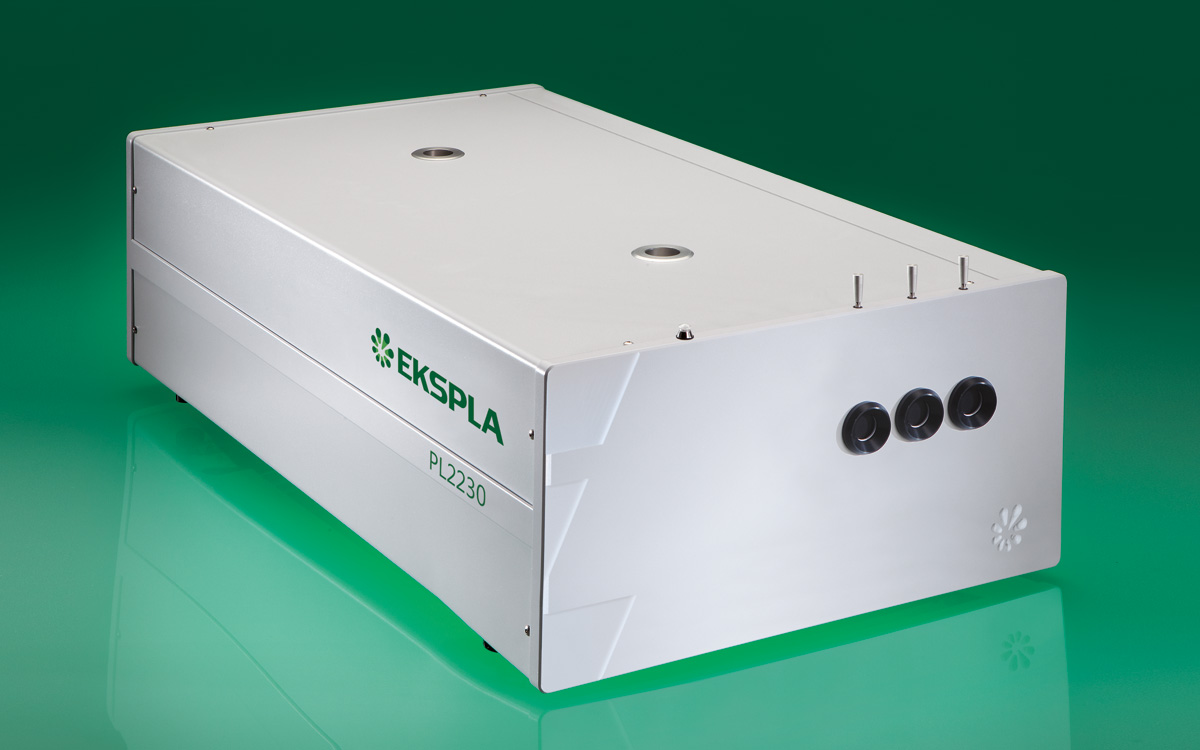
\includegraphics[width=\textwidth]{laser}
			\caption{Laser \emph{EKSPLA PL2231-50}.
% 				Převzato z~\autocite{ekspla-specs}.}
				Převzato z~\texttt{ekspla.com}.}
		\end{figure}
	\end{column}
	\end{columns}
\end{frame}

\section[E-FISH]{Electric field induced second harmonic generation}

\begin{frame}
	\frametitle{E-FISH}
	\begin{columns}
	\begin{column}{0.5\textwidth}
		\begin{itemize}
			\item \emph{electric field-induced second harmonic generation}
			\item opticky nelineární prostředí nebo vysoká intenzita
			\item $\vec\epol = \epervac (\esusn1\vec\elfield + \esusn2\vec\elfield^2
% 				+ \esusn3\vec\elfield^3
				\ldots)$
			\item $\efish = \efishconst \ndens^2 \elfieldext^2 \itylaser^2$
		\end{itemize}
	\end{column}
	\begin{column}{0.5\textwidth}
		\includegraphics[width=\textwidth]{polarization}
	\end{column}
	\end{columns}
\end{frame}

\begin{frame}
	\frametitle{Zkoumaný výboj}
	\begin{columns}
	\begin{column}{0.6\textwidth}
		\includegraphics[width=\textwidth]{efish-reactor}
		\graphicspath{{../efish/}}
		\input{../efish/results/period-overview-full-small}
	\end{column}
	\begin{column}{0.4\textwidth}
		\begin{itemize}
			\item Townsendův výboj (DBD)
			\item sklo \SI{1.1}{\milli\metre} (2\times)
			\item mezera \SI{1}{\milli\metre}
			\item elektrody \num{14}\times\SI{15}{\milli\metre}
			\item \ce{N2}, \SI{3500}{\sccm}, \SI{1}{\atmosphere}
			\item \SI{11}{\kilo\hertz}, \SI{7}{\kilo\volt},
				\SI{3}{\milli\ampere}
			\item laser \SI{50}{\hertz}
		\end{itemize}
	\end{column}
	\end{columns}
\end{frame}

\begin{frame}
	\frametitle{Uspořádání experimentu}
	\includegraphics[width=\textwidth]{efish-setup}
\end{frame}

\begin{frame}
	\frametitle{Kalibrace}
	\sisetup{per-mode=symbol}
	\graphicspath{{../efish/}}
	\input{../efish/results/period-calib-bilateral-small}
\end{frame}

\begin{frame}
	\frametitle{Výsledky}
	\begin{figure}
		\centering
		\small
		\sisetup{per-mode=symbol}
		\graphicspath{{../efish/}}
		\input{../efish/results/period-elfield-small}
		\caption{Časový vývoj intenzity elektrického pole
			v~různých místech výboje.}
	\end{figure}
\end{frame}

\end{document}
